\section{Benchmark Characterization}
\Secl{results}

The released dataset contains 9,415 Lean 4 formalization challenges (totalling 75,005 theorems) derived from 2,772 unique Python property-based tests, produced by two pipeline runs (\texttt{feb03}: 5,979 samples, Claude Sonnet 4.5; \texttt{apr08}: 3,436 samples, Claude Sonnet 4.6). Each unique PBT has between 1 and 15 formalizations. Among PBTs with multiple formalizations, 65\% have no single dominating attempt: for each formalization in the group there exists another that scores higher on at least one sub-metric of Equation~\ref{eq:faithfulness}. In practice this means, for example, that the attempt with the best assertion coverage may have worse parameter coverage than a sibling; keeping all formalizations and flagging the best one with \texttt{is\_canonical} therefore captures strictly more information than retaining only the top-scoring attempt.

\subsection{Translation Quality}

We evaluate translation quality using \emph{structural faithfulness} (Equation~\ref{eq:faithfulness}), a composite metric defined in \Secr{pipeline}. The overall faithfulness distribution (Figure~\ref{fig:faithfulness}) exhibits a clear mode above 0.5, indicating that the majority of translations preserve the essential structure of the source PBT, though a long tail of lower-quality translations remains.

In 59\% of samples the agent generated a complete Lean implementation (\texttt{Impl.lean} contains a computable definition, not just a stub); the remaining 41\% use a signature-only placeholder. Structural faithfulness is comparable across both groups (mean 0.67 vs.\ 0.68), confirming that specification quality is largely independent of whether the implementation was recovered.

The generated Lean artifacts span a wide range of complexity (Figure~\ref{fig:lean_complexity} in Appendix~\ref{appndx:complexity}): median sample contains 6 theorems with matching \texttt{sorry} counts. Per-sample pipeline cost is right-skewed (Appendix~\ref{appndx:pipeline_cost}): most samples compile within a few agent turns, but a tail of difficult translations requires many repair iterations.

\subsection{Difficulty Grading}

Each sample is graded for proof difficulty by Claude Haiku 4.5, which assigns a binary label (\emph{easy} or \emph{hard}) along with a confidence score. The benchmark contains a substantial proportion of both easy and hard problems, and the grader expresses high confidence for the majority of assessments (Figure~\ref{fig:difficulty_distribution}, Appendix~\ref{appndx:grader}). Difficulty is estimated here as a \textit{prediction}: we ask the grader to predict whether a language model agent would be able to complete the proofs successfully. Hard problems tend to produce longer Lean outputs, consistent with the intuition that more complex source PBTs lead to more elaborate formalizations and more challenging proofs (Figure~\ref{fig:difficulty_vs_faithfulness}, Appendix~\ref{appndx:grader}).

\subsection{Baselines}

\begin{figure}[t]
  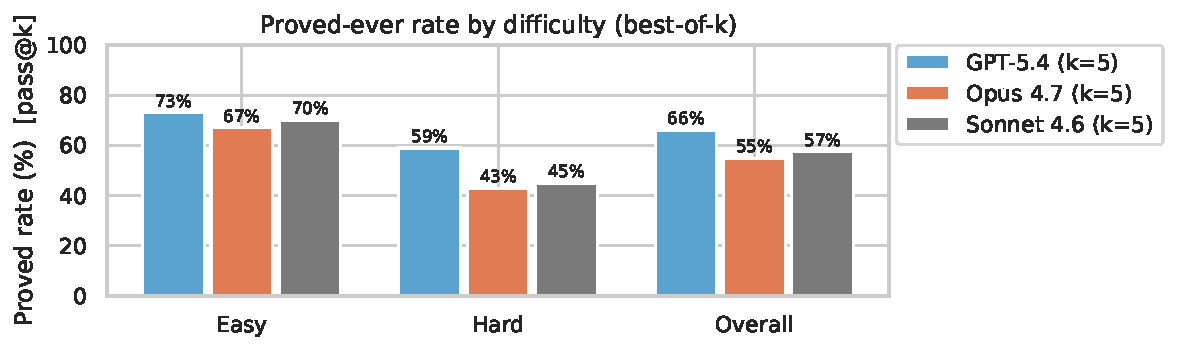
\includegraphics[width=\linewidth]{figs/baselines_prove_rate.pdf}
  \caption{Baseline prove rate}
  \label{fig:baseline_prove_rate}
\end{figure}

\begin{figure}[t]
  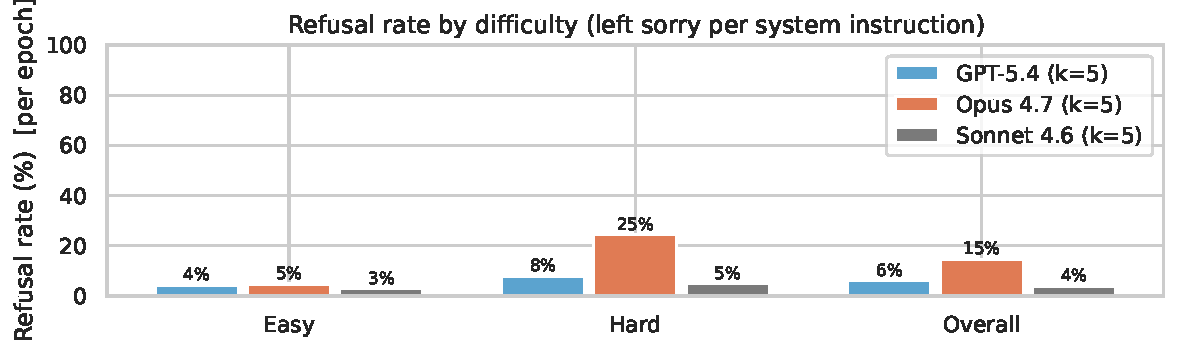
\includegraphics[width=\linewidth]
  {figs/baselines_refusal_rate.pdf}
  \caption{Baseline refusal rate}
  \label{fig:baseline_refusal_rate}
\end{figure}

We evaluate three frontier models (Claude Sonnet~4.6, Claude Opus~4.7, and GPT~5.4) on 100 randomly sampled easy problems and 100 hard problems (difficulty as defined in \Secr{results}). Each model has access to the Lean LSP via MCP tools and is scored on two metrics: a binary \emph{proved} flag (zero \texttt{sorry} remaining and \texttt{lake build} succeeds) and \emph{partial credit} (fraction of \texttt{sorry} placeholders removed).

\ref{fig:baseline_prove_rate} shows that an average of 49\% of hard samples were solved and an average of 70\% of easy samples were solved. \ref{fig:baseline_refusal_rate} is about when a language model believes a problem isn't solvable. 

\begin{figure}[t]
  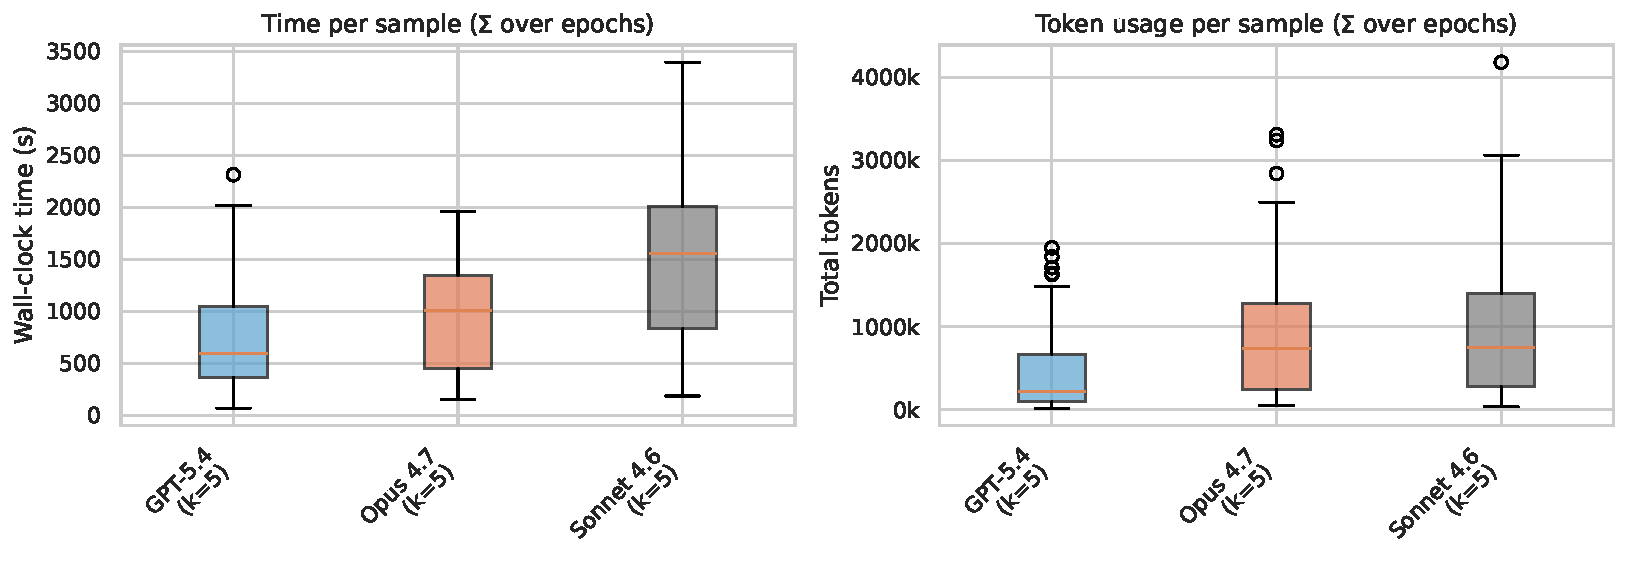
\includegraphics[width=\linewidth]{figs/baselines_cost.pdf}
  \caption{Compute cost per sample for each baseline run: wall-clock time (left) and token usage (right), summed across all attempts for $k>1$ runs. Box plots show median, IQR, and $1.5\times$IQR whiskers.}
  \label{fig:baselines_cost}
\end{figure}
